\documentclass[unknownkeysallowed]{article}
\usepackage[slovak]{babel}
\usepackage[utf8]{inputenc}
\usepackage{amsmath}
\usepackage{multicol}
\usepackage{amssymb}
\usepackage{ textcomp }
\usepackage{amsthm}
\usepackage{enumerate}
\usepackage{wrapfig}
\usepackage{graphicx}
\usepackage{listings}
\usepackage{color}
\usepackage{float}
\usepackage{indentfirst}
\usepackage{hyperref}
\usepackage{tipa}
\usepackage{mathtools}
\usepackage[top=2cm, bottom=2cm, right=2cm, left=2cm]{geometry}
\usepackage{tikz}

\newcommand\encircle[1]{%
  \tikz[baseline=(X.base)] 
    \node (X) [draw, shape=circle, inner sep=0] {\strut #1};}

\def\eps{\varepsilon}

\newtheorem{lemma}{Lema}[section]
\newtheorem{tvrdenie}{Tvrdenie}[section]
\newcommand{\liefive}{\rotatebox[origin=c]{90}{$5$}}

\title{Počítačová štatistika}
\date{}



\definecolor{mygreen}{rgb}{0,0.6,0}
\definecolor{mygray}{rgb}{0.5,0.5,0.5}
\definecolor{mymauve}{rgb}{0.58,0,0.82}

\lstset{
  backgroundcolor=\color{white},   % choose the background color; you must add \usepackage{color} or \usepackage{xcolor}
  basicstyle=\footnotesize,        % the size of the fonts that are used for the code
  breakatwhitespace=false,         % sets if automatic breaks should only happen at whitespace
  breaklines=true,                 % sets automatic line breaking
  captionpos=t,                    % sets the caption-position to bottom
  commentstyle=\color{mygreen},    % comment style
  %deletekeywords={...},            % if you want to delete keywords from the given language
  escapeinside={\%*}{*)},          % if you want to add LaTeX within your code
  extendedchars=true,              % lets you use non-ASCII characters; for 8-bits encodings only, does not work with UTF-8
  frame=single,	                   % adds a frame around the code
  keepspaces=true,                 % keeps spaces in text, useful for keeping indentation of code (possibly needs columns=flexible)
  keywordstyle=\color{blue},       % keyword style
  language=Python,                 % the language of the code
  otherkeywords={None, self},           % if you want to add more keywords to the set
  numbers=left,                    % where to put the line-numbers; possible values are (none, left, right)
  numbersep=5pt,                   % how far the line-numbers are from the code
  numberstyle=\tiny\color{mygray}, % the style that is used for the line-numbers
  rulecolor=\color{black},         % if not set, the frame-color may be changed on line-breaks within not-black text (e.g. comments (green here))
  showspaces=false,                % show spaces everywhere adding particular underscores; it overrides 'showstringspaces'
  showstringspaces=false,          % underline spaces within strings only
  showtabs=false,                  % show tabs within strings adding particular underscores
  stepnumber=2,                    % the step between two line-numbers. If it's 1, each line will be numbered
  stringstyle=\color{mymauve},     % string literal style
  tabsize=2,	                   % sets default tabsize to 2 spaces,
  title=\lstname                   % show the filename of files included with \lstinputlisting; also try caption instead of title
}

\begin{document}
\shorthandoff{-}
\maketitle

1976 -- Bell labs S - statistics (narážka na C)
1988 -- S+ -- konečná implementácia S
1997 -- R -- Eobert Gentleman, Ross Ihaka, odlíšiť od S

\section*{R-ko}
\begin{itemize}
\item attach: kópie stĺpcov v \underline{glob. namespace}
\item logické: \& , \textpipe , $==$, $!=$, !
\item order: vektor pozícií v poradí
\item rank: pozície v usp. poli
\item data.frame: matica objektov
\item Ctrl+R -- run
\item vektory = stĺpce
\item násobenie matíc: \%*\%
\item $solve(A,\vec{v}) \rightarrow$ riešenie $A\vec{x} = \vec{v}$
\item objekt\$param -- stĺpec
\item NAN - not a number
\item NA - not available = chýbali dáta
\item imputačná technika -- okus nahradiť NA nejakými dátami
\item FACTORS -- premenné, ktoré nie sú číselné, LEVELS OF FACTOR -- hodnoty tejto premennej( set: M,F )
\item table -- kontingenčná tabuľka
\end{itemize}

\section*{Štatistiky a variability}

\begin{figure}[ht]
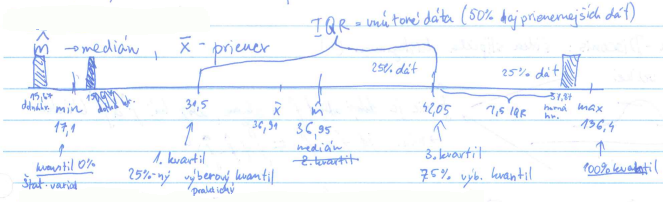
\includegraphics[width=\textwidth]{imgs/obr1.png}
\centering
\end{figure}

\begin{itemize}
\item $S^2$ -- variabilita dát
	\begin{itemize}
		\item význam má hlavne pri porovnávaní 2 vzoriek dát
		\item v štat. na normalizácie
	\end{itemize}
\item IQR -- interquartile range -- uchopiteľnejšie ako $S^2$
\item dolná hradba = 1. kvantil -- 1.5*IQR : prečo 1.5? -- určuje šírku hradieb -- pre bežné \underline{dáta funguje}\footnote{nie sú príliš úzke ani široké}
\item outliers $\to$ mimo hradieb $\to$ treba sa pozrieť na to, ako vznikol? $\to$ zaradiť \& vyhodiť (chyba meranie)
	\begin{itemize}
	\item ak ich necháme, robí sa analýza s out. aj bez out. samostatne
	\end{itemize}
\end{itemize}

\subsection*{Obrázky}
Lotéria: všetci si stavili číslo 0-999, tí čo si tipli vyžrebované si rozdelili peniaze

\begin{itemize}
\item Boxplot: outliers
\end{itemize}

\begin{figure}[ht]
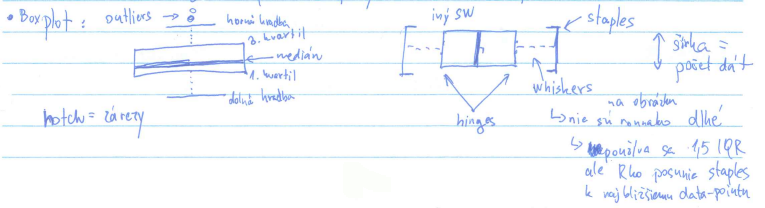
\includegraphics[width=\textwidth]{imgs/obr2.png}
\centering
\end{figure}

%\begin{wrapfigure}{r}{0.5\linewidth}
%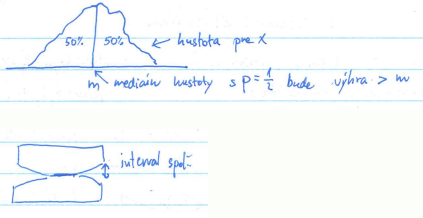
\includegraphics[width=\linewidth]{imgs/obr3a4.png}
%\end{wrapfigure}

\subsubsection*{Zárezy}


X -- náhodná premenná 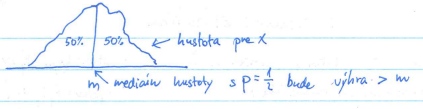
\includegraphics[width=0.5\linewidth]{imgs/obr3.png}

\vspace{5mm}

\begin{multicols}{2}
odhady pre $m$:
\begin{enumerate}
\item bodový odhad: \^{m} \ldots medián z dát (výberový)
\item intervalový odhad: IS pre $m$: \^{m} $\pm$ čosi
\end{enumerate}
\columnbreak
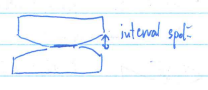
\includegraphics[width=0.5\linewidth]{imgs/obr4.png}
\end{multicols}

\vspace{5mm}
Boxploty sa vždy maľujú viaceré

Medián je \underline{robustný} = odolný voči outlierom \qquad 5,1,1,2,1 $\to$ $\Phi = 2 \land \hat{m} = 1$

\vspace{5mm}

medián + priemer: Viac ako polovica Slovákov má podpriemernú mzdu:
\begin{center}
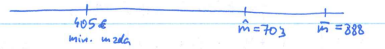
\includegraphics[width=0.5\linewidth]{imgs/obr5.png}
\end{center}

Norm. rozdelenie $N(0,1) \qquad f(x) = \frac{1}{\sqrt{2\pi}}e^{\frac{-x^2}{2}}$

Cauchyho rozdelenie $f(x) = \frac{1}{2\pi}\frac{1}{1+x^2}$

\vspace{5mm}
Freedman-Diaconis: šírka stĺpčeka histogramu (n)

pre $a)$ aj $b)$: $\hat{f}$ nie je dobrý odhad $f$ -- chceme, aby boli $f$ a $\hat{f}$ blízko -- min. vzd. $f$ a $\hat{f}$ = $\int_{-\infty}^{\infty}{(\hat{f}-f)^2}$
\begin{enumerate}
\item[a)] $h$ je veľké


\includegraphics[width=0.5\linewidth]{imgs/obr6.png}
\item[b)] $h$ je malé $\to$ pre veľkú triedu funkcií je riešením práve $h=2\cdot IQR\cdot n^{-\frac{1}{3}}$


\includegraphics[width=0.5\linewidth]{imgs/obr7.png}
\end{enumerate}

\section*{Rozdelenia a hustoty v R}
\begin{multicols}{2}
\begin{itemize}
\item \texttt{dnorm(x, mean=4, sd=30)}
	\begin{itemize}
	\item \textbf{d}norm = density
	\item d\textbf{norm} = norm. rozdelenie
	\item mean=4, sd=3 \ldots hustota $N(4,9)$, dke 9 je $\sigma^2$
	\end{itemize}
\item \texttt{pnorm(7)} = distrib. f. v 7 $= F(7) = P[x<7]$
	\begin{itemize}
	\item \textbf{p}norm = probabilty
	\end{itemize}
\item \texttt{qnorm(0.09)} = 9\% kvantil
	\begin{itemize}
	\item \textbf{q}norm = quantile
	
	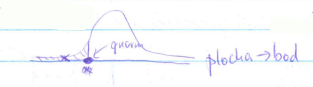
\includegraphics[width=\linewidth]{imgs/obr9.png}
	\end{itemize}
\item \texttt{rnorm(103)} -- vygeneruje sa $x_1, \ldots, x_{103} \sim N(0,1)$ a sú IID
\end{itemize}
\columnbreak
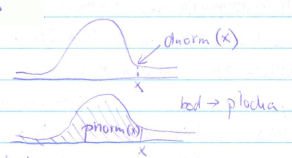
\includegraphics[width=\linewidth]{imgs/obr8.png}
\end{multicols}

POZN: množstvo štat. metód vyžaduje ďalšie generovanie dát
\begin{multicols}{2}
\begin{itemize}
\item[-] \texttt{norm} -- \underline{normálne rozdelenie}
\item[-] \texttt{t(\ldots, df)} - \underline{Studentovo rozdelenie} $t_{df}$, df = degrees of freedom
\item[-] \texttt{chisq(\ldots, df=4)} -- $\chi_4^2$ -- \underline{chi kvadrát}
\item[-] \texttt{f(\ldots, df1=2, df2=8)} -- \underline{Fischerovo-Schnedekerovo rozdelenie}
\end{itemize}
\columnbreak
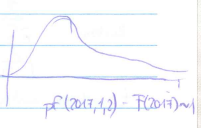
\includegraphics[width=0.7\linewidth]{imgs/obr10.png}
\end{multicols}

\section*{Sklon dát}
Väčšina dát je z norm. rozdelenia, ale \underline{treba overiť}!

\begin{multicols}{2}
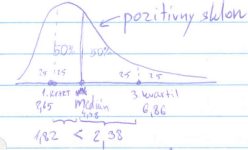
\includegraphics[width=0.7\linewidth]{imgs/obr11.png}

pozitívny sklon: $(3\hat{k}-\hat{m}) > (\hat{m}-1\hat{k})$


(jednoduchšie, ale dáta treba usporiadať)
\columnbreak

{pozitívny sklon -- ako to matematicky zistiť?}

\begin{equation*}
\mathrm{skewness} := \dfrac{\sum\limits_{i=1}^{n}{(x_i-\bar{x})^3}}{\left[\sum\limits_{i=1}^{n}{(x_i-\bar{x})^2}\right]^{\frac{3}{2}}}
\end{equation*}

\begin{itemize}
\item $skewness>0$ -- pozitívny sklon
\item $skewness=0$ -- symetrická hustota
\item $skewness<0$ -- negatívny sklon
\end{itemize}
\end{multicols}

\paragraph{Q-Q plot} (Quantile-Quantile plot -- \underline{kvantilový diagram})

y-ové súradnice guľôčok sú usporiadané dáta $x_{(1)} < x_{(2)} < \ldots < x_{(1000)}$

x-ové súradnice kvantily $N(0,1)$ \qquad $kvantil(\frac{1}{1000+1}) < kvantil(\frac{2}{1000+1}) < \ldots < kvantil(\frac{1000}{1000+1})$

\begin{figure}[ht]
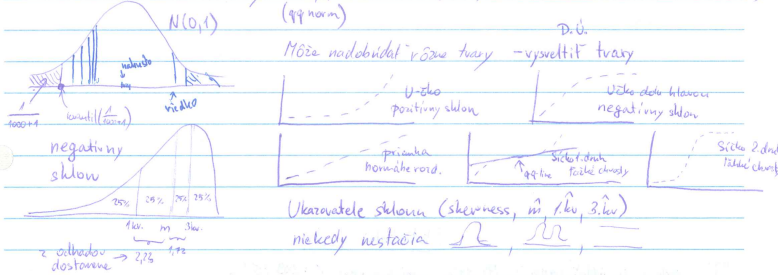
\includegraphics[width=\textwidth]{imgs/obr12.png}
\centering
\end{figure}

qqline -- priamka cez body $\frac{1}{4}, \frac{3}{4}$

\begin{itemize}
\item Esíčkový kv. diagram \textbf{1. druhu}: Dáta pochádzajú z hustoty, ktorá má \underline{ťažšie chvosty} než $N(\ldots, \ldots)$, a teda špicatejší kopček než $N(\ldots, \ldots)$
\item Esíčkový kv. diagram \textbf{2. druhu}: Dáta sú z rozdelenia s hustotou s \underline{ľahšími chvostami} a mohutnejším kopčekom
\end{itemize}

\begin{figure}[H]
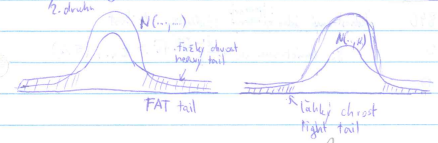
\includegraphics[width=\textwidth]{imgs/obr13.png}
\centering
\end{figure}

\paragraph{\underline{KURTOSIS}} (vydutosť) -- výberový keoficient špicatosti

\begin{equation*}
\mathrm{kurtosis} := \dfrac{\sum\limits_{i=1}^{n}{(x_i-\bar{x})^4}}{\left[\sum\limits_{i=1}^{n}{(x_i-\bar{x})^2}\right]^{2}}
\end{equation*}

\begin{itemize}
\item $kurtosis>3$ -- špicatejší kopček, ťažšie chvosty
\item $kurtosis=3$ -- dáta sú z norm. rozdelenia
\item $kurtosis<3$ -- mohutnejší kopček, ľahšie chvosty
\end{itemize}

teoretická kurtosis -- získame ju z hustoty:
\begin{equation*}
\dfrac{E[(X-E(x))^4]}{E[(X-E(x))^2]^2} = 3
\end{equation*}

Rovná sa 3, bez ohľadu na $\mu$ a $\sigma^2$. Menovateľ je $\sigma^{2^2}$. Ešte treba ukázať, že čitateľ je $3\sigma^4$.

reálne dáta -- hľadáme \underline{hsutotu}, ktorá sa najviac podobá na naše dáta
\begin{itemize}
\item[-] metóda: histogram (schodíkový odhad)
\item[-] \underline{jadrové odhady} (kernel estimates) -- v Rku density
\end{itemize}

Obrázok -- histogram, gauss, kernel estimate $\to$ ak sa podobá kernel est na gaussa, pravdepodobne to bude norm. rozdelenie

\paragraph{Historické príklady falšovania dát}
\begin{itemize}
\item[-] franc. profesor -- hoďťe mincou 1000 krát a odovzdajte zápis
	\begin{itemize}
	\item[-] pomer 500:500 sa im podarilo napodobniť
	\item[-] tí čo podvádzali nemali dlhé rovnaké sekvencie
	\end{itemize}
\item[-] Mendel (brnenský mních, objavil zákony dedičnosti) -- kríženie hrachov s bielymi a zelenými kvetmi
	\begin{multicols}{2}
	\begin{itemize}
	\item[-] pozrel sa na dáta Fischer (štatistik) -- zákon síce platil, ale experimenty (veľa hrahov) sú falšované
	\item[-] 100 hrachov na 1 políčku: 26:47, 25:75, 24:76 -- skutočné pomery by boli ďalej od 25:75 -- ukázal pomocou \underline{testu dobrej zhody}
	\item[-] pravdepodobne za to môže pomocník: zatajil výsledky 85:15 $\to$ \underline{CONFIRMATION BIAS} -- zbieranie len dát, ktoré potvrdzujú hypotézu
	\end{itemize}
	\columnbreak
	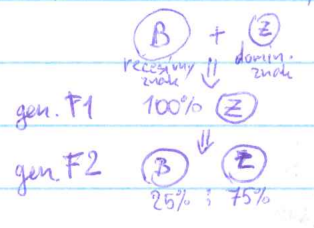
\includegraphics[width=0.2\textwidth]{imgs/obr14.png}
	\end{multicols}
\end{itemize}

\section*{Štatistické testy}
1878: verilo sa, že rýchlsoť svetla je $299~840$, Michelsonov $\bar{X} = 299~852,4$

$X_1,\ldots,X_{n=100} \sim N(\mu, \sigma^2)$, $\mu$ nepoznáme = skutočná rýchlosť svetla

Spravíme Studentov t-test

$$H_0: \mu \leq 840 \qquad vs. \qquad H_1: \mu > 840 ~\mathrm{(research~hypothesis)}$$

\subsection*{One-sided t-test}
MZR: $H_0$ zamietame ak $\bar{X} >> 840$. Jednostranný súborový studentov t-test.

\begin{multicols}{2}
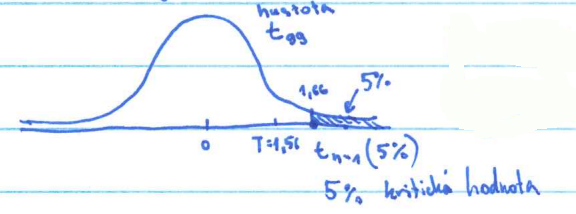
\includegraphics[width=0.5\textwidth]{imgs/obr15.png}
\columnbreak

$H_0$ zamietame ak $T=\frac{\bar{X}-840}{S}\sqrt{n} > t_{n-1} (5 \%)$
\end{multicols}

t-test v Rku: \texttt{t.test(Y, alternative=greater, mu=840)}

$t = T = \frac{\bar{X}-840}{S}\sqrt{n} = 1.5694$ chýba tu kritická hodnota $t_{99}(5\%) \to$ Rko nevie robiť krit. hodnoty ako kvantily

\begin{multicols}{2}
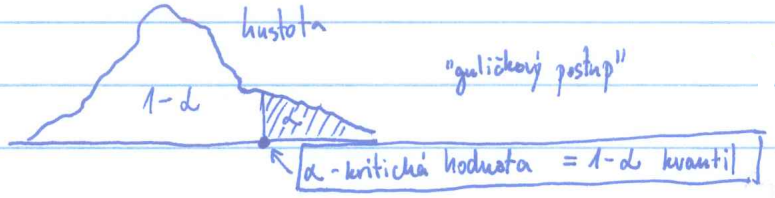
\includegraphics[width=0.5\textwidth]{imgs/obr16.png}
\columnbreak

$T \ngtr t_{99}(5\%) \qquad t_{99}(5\%) = 1.66$

-- hypotézu $H_0$ nezamietame
\end{multicols}

-- Mechelspon nemôže tvrdiť, že $c > 299~840$, Studentov t-test zohľadnil
\begin{enumerate}
\item rozdiel 840 a 852 je dosť malý
\item vzorka 100 dát je malá
\item dáta sú rozdistribuované
\end{enumerate}

p-value $\in <0,1>, \qquad p=5.98\%$ -- plocha od $T\to\infty$

Ak p-value $<5\%$, $H_0$ zamietame, ak p-value $>5\%$, $H_0$ nezamietame

\begin{itemize}
\item ``p-value'' -- porovnaj $t$ a $T$
\item ``guľičkový postup'' -- porovnaj plochy 5\% a $\int_T^{\infty}{p(x)dx}$
\end{itemize}

\subsection*{Two-sided test}
TRUE: $299~792~km/h$ -- Porovnáme Michelsonove dáta s realitou

$$H_0: \mu = 792 \qquad vs. \qquad H_1: \mu \neq 792$$

MZR: $H_0$ zamietame ak $\bar{X} >> 792$ alebo ak $\bar{X} << 792$.

\begin{multicols}{2}
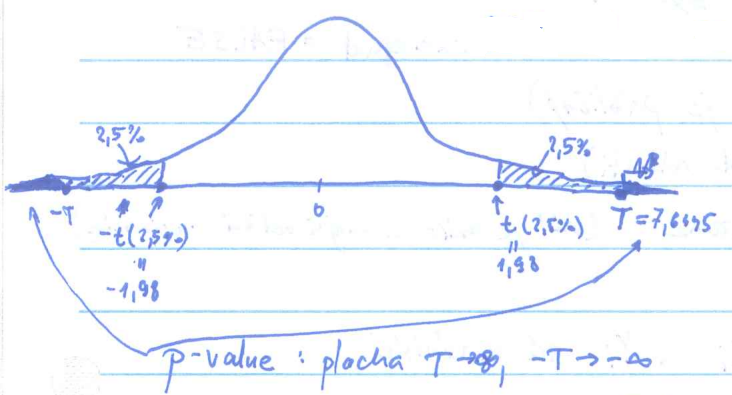
\includegraphics[width=0.5\textwidth]{imgs/obr17.png}
\columnbreak

\begin{align*}
\bar{X} >> 792&\mathrm{~alebo~}\bar{X} << 792\\
\bar{X}-792 >> 0&\mathrm{~alebo~}\bar{X}-792 << 0\\
T = \frac{\bar{X}-792}{S}\sqrt{n} > t(2.5\%)&\mathrm{~alebo~}<-t(2.5\%)\\
7.6445 > 1.98&\mathrm{~alebo~}7.6445 < -1.98
\end{align*}

\end{multicols}

Zamietame $H_0$, problém! -- systematická chyba merania, michelson dostáva dáta s $\mu > c$.

\subsection*{Ešte jeden 1-stranný t-test}
V 1878 sa verilo, že NEWCOMBE: 860 \qquad (MICHELSON: 852.4 $\to$ bol bližšie k TRUE: 792)

$$H_0: \mu \geq 860 \qquad vs. \qquad H_1:  \mu < 860$$

\begin{multicols}{2}
$H_0$ zamietame ak $\bar{X} << 860$

\begin{align*}
&T = \frac{\bar{X}-860}{S}\sqrt{n} &&< -t(5\%) = t(95\%)\\
&-0.9619 &&> -1.66
\end{align*}

$H_0$ zamietame, test nie je štatisticky významný

p-value = $p(\tau < -0.96) = F_T(-0.96)$

\columnbreak

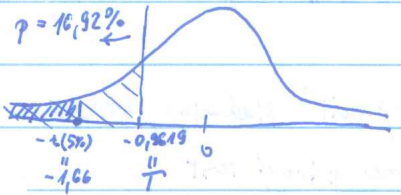
\includegraphics[width=0.5\textwidth]{imgs/obr18.png}
\end{multicols}

\paragraph{Dva dni meraní pre rýchlosť svetla}~

$X_1, \ldots, X_n \sim N(\mu_x, \sigma^2)$

$Y_1, \ldots, Y_n \sim N(\mu_y, \sigma^2)$

predpokladáme, že sigmy sú rovnaké, ale treba to overiť

$\mu_x$ a $mu_y$ -- skutočné rýchlsoti svetla v určitých dňoch:

$$H_0: \mu_x = \mu_y \qquad vs. \qquad H_1:  \mu_x \neq \mu_y$$

\underline{Predtest:} $H_0: \sigma^2_x = \sigma^2_y \qquad vs. \qquad H_1:  \sigma^2_x \neq \sigma^2_y$

MZR: $H_0$ zamietame ak $S_x^2 >> S_y^2$ alebo $S_x^2 << S_y^2$.

F-test: $\frac{S_x^2}{S_y^2} >> 1$ alebo $\frac{S_x^2}{S_y^2} << 1$ (var. test)

2. a 4. deň $\frac{S_x^2}{S_y^2}=F=1.0377 \qquad p-value = 93\% \Rightarrow H_0$ nezamietame :)

\subsection*{2-výberový Studentov t-test}
$H_0$ zamietame ak $\mu_x >> \mu_y$ alebo $\mu_x << \mu_y$ \qquad \texttt{var.equal=TRUE} $\to$ predtest dopadol dobre

p-value = $7.17\% > 5\%$, teda $H_0$ nezamietame

$\to$ t-test povedal, rozdiel ($\bar{X}=856, \bar{Y}=820.5$) nie je štatisticky významný lebo vzorka 20 dát je málo

\subsection*{2-výberový Welchov t-test}
1. a 2. deň		$H_0: \sigma_x^2 = \sigma_y^2 \qquad vs. \qquad H_1: \sigma_x^2 \neq \sigma_y^2 \qquad \frac{S_x^2}{S_y^2} = 2.9$ :(

$\to$ 2-výverový Welchov t-test \qquad \texttt{var.equal=FALSE}
\begin{enumerate}
\item $T = \frac{\bar{X}-\bar{Y}}{\sqrt{\ldots}} \dot{\sim} t_\nu$ (tento test je približný)
\item $\nu = ?$, treba ho odhadnúť (\#st. voľnosti)
\end{enumerate}

p-value = 6\%, $H_0: \sigma_x^2 = \sigma_y^2$ nezamietame (dát je málo a majú veľkú varianciu)

\subsection*{Párový t-test}
Predpoklad St. t-testu a Welchovho t-testu: dáta $X_i$ a $Y_i$ sú nezávislé

Dáta podrážok: opotrebovanie pred a po nosení, rozdiel je 1 číslo
-- $\forall$ dieťa nosilo topánku A aj B, porovnávame opotrebovanie \qquad materialA: X \qquad materialB: Y

$$H_0: \mu_x \leq \mu_y \qquad vs. \qquad H_1: \mu_x > \mu_y \mathrm{~(research~hypothesis)} $$

Hypotéza: A sa opotrebováva viac ako B.

Nemôžeme spraviť studentov, welchov t-test, lebo \underline{dáta nie sú nezávislé} (v stĺpcoch, pravá/ľavá topánka).

$\to$ použijeme párový test $\to$ dáta v dvojiciach $\binom{X_1}{Y_1}\ldots\binom{X_n}{Y_n} \sim N_2\left(\binom{\mu_x}{\mu_y}, \left(\begin{matrix}
  \sigma_x^2 & cov \\
  cov & \sigma_y^2
 \end{matrix}\right)\right)$
 
\begin{enumerate}
\item párovanie\footnote{Stačí overiť že rozdiely $Z \sim N$} $Z_i = X_i - Y_i \sim N(\mu_x-\mu_y), (1, -1)\left(\begin{matrix}
  \sigma_x^2 & cov \\
  cov & \sigma_y^2
 \end{matrix}\right)\binom{1}{-1} = \sigma_x^2 + \sigma_y^2 - 2cov)$
\item 1-súborový studentov t-test na dátach $Z_1, \ldots, Z_n$, ($T = \frac{\bar{Z}-0}{S}\sqrt{n} > t_{n-1}(5\%)$)
\end{enumerate}

Ak do t-testu dáme závislé dáta, bude sa správať \underline{konzervatívne}, vysoká p hodnota

\vspace{5mm}

Ako Mechelson meral rýchlosť svetla?

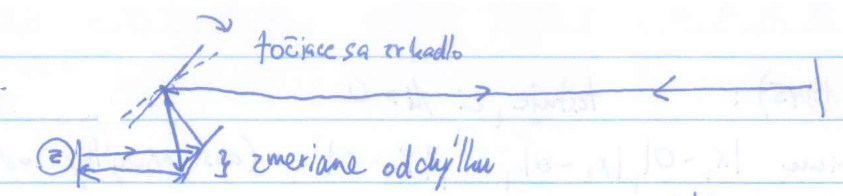
\includegraphics[width=0.5\textwidth]{imgs/obr19.png}

problémy: kým svetlo prešlo tam a naspäť, zrkadlo sa veľmi nestihlo pohnúť

(Poliak) $\to$ rýchlejšie potreboval roztočiť zrkadlo $\to$ použil parný stroj = zdroj nepresností (nestále otáčky)

-- prvý Američan, ktorý získal Nobelovu cenu za vedu

\section*{Testy normality}
\subsection*{Kolmogor-Smirnov test}
$X_1, \ldots, X_n \overset{?}{\sim} N(,)$ \qquad $H_0: \mathrm{data} \sim N(\ldots,\ldots) \qquad vs. \qquad H_1: \mathrm{data~nie~su~z} N(\ldots,\ldots)$

dáta pochádzajú z rozdelenia, ktoré má \underline{distribučnú funkciu}\footnote{CDF: Cumulative Distribution Function} $F(\ldots) = ?$ (nepoznáme ju)

$\to$ odhad $F(7) = P(X<7) = \frac{\#\{x_i < 7 \}}{n} =: \hat{F}(7) \cdots$ ECDF: Empirical CDF

Idea testu: Ak platí $H_0$, tak ECDF $\hat{F}(\ldots)$ by sa mala podobať na CDF pre $N(\mu, \sigma^2)$ (pnorm). Za $\mu$ zvolíme $\bar{X}$, za $\sigma^2$ zvolíme $S^2$.

\begin{multicols}{2}
$H_0$ zamietame ak $\hat{F}$ a pnorm($\bar{x}, S$) sú veľmi oslišné.

D: maximálna zvislá odchýlka $ >> 0$ (test. štatistika)

p-hodnota: D sa riadi nejakým rozdelením $\to$ Kolmogorov-Smirnov ho zrátali

pre rýchlsoť svetla $p=45\% >> 5\%$, $H_0$ nezamietame

\columnbreak

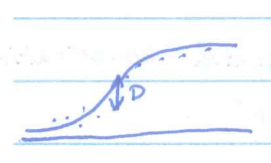
\includegraphics[width=0.2\textwidth]{imgs/obr20.png}

\end{multicols}

\subsection*{Shapirov-Wilkov test (pre malé sady dát)}
-- snaží sa zistiť, či kvantilový diagram vyzerá ako praimka

Žiaden test normalitu $Z_i$ (podrážky dáta A - dáta B) nezamietal napriek tomu, že histogram naznačuje, že dáta nie sú normálne, ale vznil \underline{z 10 dát}.

\section*{Neparametrické testy}
Levi-Strauss -- testovali naraz nanášanie farby ľuďmi vs. strojmi an látku

-- dáta:  \% nepodarkov ľudia-stroje $\to$ o koľko \% sa ľudia viac mýlili

$\to$ dát je len 22, ale napriek tomu SW test normalitu zamieta
\qquad $\to$ je tam veľa outlierov, pri normálnom rozdelení by mali byť približne $\frac{1 out.}{100 dat}$.

$X_1, \ldots, X_n \nsim N()$

$?\mu = E(X)$ -- stredná hodnota nepodarkov ľudí voči strojom

$$H_0: \mu \leq 0 \qquad vs. \qquad H_1: \mu > 0$$

$H_1$ = ľudia sú horší ako stroje

--nemôžeme použiť Studentov t-test (nemáme $N$)

\subsection*{Wilcoxon(1945)}
testuje, či $\mu > 0$
\begin{enumerate}
\item Zoberieme $|X_1 - 0|, |X_2 - 0|, \ldots, |X_n - 0|$ (abs. odchýlky od strednej hodnoty)
\item orankujeme odchýlky $\ldots n \ldots 2 \ldots 1 \ldots 3 = R_1 \ldots R_n$
\item $S_W = \sum_{i,x_i-0 > 0} R_i$ (súčet rankov, kde bola odchýlka kladná), $H_0$ zamietame ak $S_W >> 0$.
\end{enumerate}

$X_1, \ldots, X_m \nsim N(,)$ a $Y_1, \ldots, Y_n \nsim N(,)$

$$H_0: \mu_x = \mu_y \qquad vs. \qquad H_1: \mu_x \neq \mu_y$$

sú navzájom nezávislé
\begin{enumerate}
\item jedna sada dát: $X_1, \ldots, X_m, Y_1, \ldots, Y_n$
\item Ranky: $\ldots 1 \ldots 3 \ldots 2 \ldots m+n = R_1, \ldots R_m, R_{m+1}, \ldots, R_{m+n}$
\item $S_W = \sum_{i=1}^m R_i$ -- sčítame len ranky $X$-ov
\end{enumerate}
-- netreba overovať rovnosť disperzií

Ak do t-testu vložíme nenormálne dáta (majú veľa outlierov), t*test sa správa konzervatívne. Ak test $\sigma_1^2 \overset{?}{=} \sigma_2^2$ dopadne tesne k 5\% $\to$ skúsime Welch $\to$ nebude fungovať

B.D.Ú. o 2 roky po Wilcoxonovi: MANN, WHITNET 1974 vymysleli ešte jednoduchší postup, všetky dvojice $X_i \overset{>}{\underset{<}{=}} Y_j$, test. štatistika $S_{MN} := \# pripadov\{ x_i > y_j \}$

\qquad -- je ich $m\cdot n$

\qquad -- Wilcoxonova test. štatistika - MANN, WHITNEY = konštanta
\begin{enumerate}
\item Zistiť, čomu sa daná konštanta rovná
\item Dokázať, že naozaj bude rovnaká pre $\forall$ prípady
\end{enumerate}
štat. môže závisieť od $n,m$, nebude závisieť od konkrétnych dát

\underline{Sestry a rukavice -- používajú ich zdravotné sestry pri práci s krvou?} tajne ich sledovali

školenie $\to$ potom znovu prieskum o 1 mesiac
\begin{itemize}
\item 2 mesiace $\to$ horšie
\item 5 mesiacov $\to$ ako keby šklenie ani nebolo
\end{itemize}

\underline{Bernoulliho schéma} -- opakujeme stále ten istý experiment s pravdep. $p$ (áno/nie) $\to$ \underline{binomické rozdelenie}

$X \sim Bin(n,p)$, X -- koľkokrát ich použili?, $n$ - \# sledovaní vrámci obdobia, $p$ - svedomitosť sestier - nepoznámne (všetkých/priemerne)

\paragraph{1-stranný test}~\\
$X = \sum$kedy nosili, $\hat{p} = \frac{x}{n}$\\
$n = $ \# pozorovaní

v New Yourku je priem, svedomitosť 20\%

$$H_0: p \leq 0.20 \qquad vs. \qquad H_1: p > 0.20$$

MZR: $H_0$ zamietame ak $\hat{p} >> 0.2$, teda $\hat{p}-0.2 >> 0$, teda $\frac{\hat{p}-0.2}{\sqrt{\frac{\hat{p}(1-\hat{p})}{n}}} > u(5\%)$, vtedy $H_0$ zamietame.

$X \sim Bin(n,p) \leftarrow$ ďalej: akým rozdelením sa riadi $\hat{p}-0.2$?
\begin{enumerate}
\item LAPLACE-MOIVRE CLT: $\frac{x-np}{\sqrt{np(1-p)}} \dot{\sim} N(0,1)$
\item MMS: $\frac{\frac{1}{n}}{\frac{1}{n}}\frac{\frac{x}{n}-p}{\sqrt{\frac{p(1-p)}{n}}} \dot{\sim} N(0,1)$
\item BDU: treba dokázať $\frac{\hat{p}-p}{\sqrt{\frac{p(1-p)}{n}}} \dot{\sim} N(0,1)$
\end{enumerate}

\begin{multicols}{2}
p-value = $1-F(v) = 0.18 > 5\%$ $\Rightarrow$ $H_0$ nezamietame

Mali sme tušenie, že priemer našich sestier je väčší ako newyorský.

Ale nie je to štat. významné:

rozdiel 20\% a 25\% je malý, n = 51 je málo dát

\columnbreak
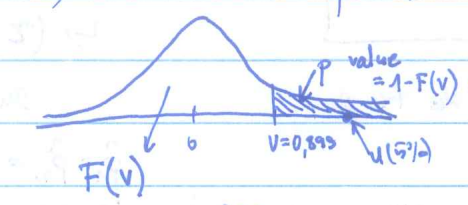
\includegraphics[width=0.3\textwidth]{imgs/obr21.png}
\end{multicols}

\paragraph*{obojstranný test}~\\

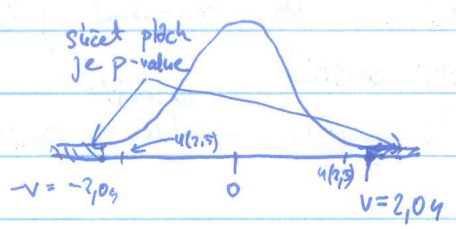
\includegraphics[width=0.3\textwidth]{imgs/obr22.png}

v USA je priemer svedomitosti 13\%

$$H_0: p = 0.13 \qquad vs. \qquad H_1: p \neq 0.13$$

MZR: $H_0$ zamietame, ak $\hat{p} >> 0.13$ alebo $\hat{p} << 0.13$. $H_0$ zamietame, ak $\frac{\hat{p}-0.13}{\sqrt{\frac{\hat{p}(1-\hat{p})}{n}}} > u(2.5\%)$ alebo $ < (2.5\%)$.

p-value = $4\% < 5\% \Rightarrow $ $H_0$ zamietame, $H_1: p \neq 0.13$.

\underline{Čo je to p-value?}

Čo si ľudia myslia: keď $p<5\%$, tak $H_0$ zamietame. AK $p>5\%$, $H_0$ nezamietame. $H_0$ platí nie je náhodá udalosť.

p-value: je pravdepodobnosť, že testovacia štatistika by vyšla ešte väčšia/menšia (extrémnejšia) ako teraz.

\subsubsection*{Interval spoľahlivosti}

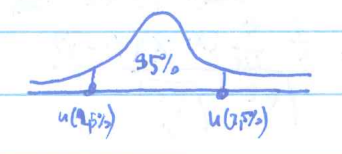
\includegraphics[width=0.3\textwidth]{imgs/obr23.png}

$$P(-u(2.5\%) < \frac{\hat{p}-p}{\sqrt{\frac{\hat{p}(1-\hat{p})}{n}}} < u(2.5\%)) = 95\%$$
$$P(\hat{p}-u(2.5\%)\sqrt{\frac{\hat{p}(1-\hat{p})}{n}} < p < \hat{p} + u(2.5\%)\sqrt{\frac{\hat{p}(1-\hat{p})}{n}}) = 95\%$$
$$L = 0.135 < p < U = 0.374$$

-- skutočná svedomitosť $\in (13\%, 37\%)$, $\hat{p} = 0.254$ -- stred intervalu

\vspace{5mm}
\underline{Závisí svedomitosť od skúsenosti?}

$X_1 \sim Bin(n_1, p_1 = ?)$ najviac 3 roky, $\hat{p_1} = \frac{7}{10}$

$X_2 \sim Bin(n_2, p_2 = ?)$ najviac 3 roky, $\hat{p_2} = \frac{6}{41}$

\vspace{5mm}
\underline{2-sample 2-sided test}

\begin{multicols}{2}

$H_0: p_1=p_2 \qquad vs. \qquad H_1: p_1 \neq p_2$\\
MZR: $H_0$ zamietame ak $\hat{p}_1 >> \hat{p}_2$ alebo $\hat{p}_1 << \hat{p}_2$\\
$H_0$ zamietame ak $\hat{p}_1 - \hat{p}_2 >> 0$ alebo $<< 0$\\
$V > u(2.5\%)$ alebo $<-u(2.5\%)$

\columnbreak

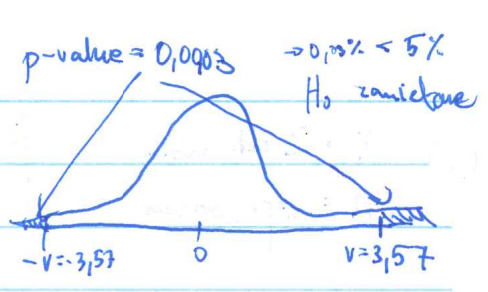
\includegraphics[width=0.3\textwidth]{imgs/obr24.png}

\end{multicols}

$$V = \frac{(\hat{p}_1 - \hat{p}_2) - (p_1 - p_2)}{\sqrt{\frac{\hat{p}_1(1-\hat{p}_1)}{n_1} + \frac{\hat{p}_2(1-\hat{p}_2)}{n_2}}}$$

Dá sa odvodiť rovnako ako 1-sample.

Je to štatisticky významné meranie svedmitosti $\to$ (z 1-str. testu potom zistíme, že menej skúsené sú svedomitejšie)

$\hat{p}_1 - \hat{p}_2 = 0.554$ -- bodový odhad

IS $P(-u(2.5\%) < V < u(2.5\%)) = 95\%$

$P(\hat{p}_1 - \hat{p}_2 - \sqrt{\frac{\hat{p}_1(1-\hat{p}_1)}{n_1} + \frac{\hat{p}_2(1-\hat{p}_2)}{n_2}}u(2.5\%) < p_1 - p_2 < \hat{p}_1 - \hat{p}_2 + sqrt{\frac{\hat{p}_1(1-\hat{p}_1)}{n_1} + \frac{\hat{p}_2(1-\hat{p}_2)}{n_2}}u(2.5\%) )$

IS = (0.249; 0.857) -- možno sú len o 25\% menej svedomité

$\to$ prečo vyšiel taký široký? : v prvej skupine(neskúsených sestier) máme len 10 pozorovaní

$X \sim Bin(n, p)$ -- je rozumné predpokladať, že každá sestra v nemocnici má rovnaké $p$?

$\to$ mohli by sme uvažovať $p$ pre každú sestru zvlášť (logistická regresia -- príliš zložité)

$\to$ je to ale až taká volovina? davová psychóza $\to$ dav sa zuniformuje

Robert Box: ``Every model is wrong, but some are useful.''

\section*{Korelačná analýza}

$\left(\begin{matrix}
  X\\
  Y
 \end{matrix}\right)\begin{matrix}
  - & INCOME\\
  - & FROST
 \end{matrix}$
 
\subsection*{PEARSON corelation coef.}

$$\rho := \frac{cov(X,Y)}{\sqrt{D(x)}\sqrt{D(Y)}} = \frac{E((X-E(x))(Y-E(Y)))}{\sqrt{D(X)}\sqrt{D(Y)}} = \frac{\int_{-\infty}^{\infty} \int_{-\infty}^{\infty}(X-E(X))(Y-E(Y))f(x,y)dxdy}{\sqrt{D(X)}\sqrt{D(Y)}} = ?$$

Kde $f(x,y)$ je združená hustota vektora $\binom{X}{Y}$. NIKDY to ale nezrátame.

Dáta $\binom{X_1}{Y_1} \cdots \binom{X_n}{Y_n} \to$ odhad pre $\rho : \hat{\rho} := \frac{\frac{1}{n}\sum_{i=1}^n{(x_i-\bar{x})(y_i-\bar{y})}}{\sqrt{S_x^2}\sqrt{S_y^2}} \in <-1,1>$.

\texttt{cor(Income, Frost) = 0.22} $\to$ lebo bohatšie regióny sú na S/SV -- nie je to kauzalita

\texttt{cor(Murder, Life Ex) = -0.87} $\to$ nie, že by sa vraždili $\Rightarrow$ krátky život/ale je tam zlá situácia (vraždy/krátky živ)

$\qquad\to$ sú to len dohady $\hat{\rho}$ -- nerobiť závery len na tom $\to$ TEST

\subsection*{Testy významnosti korelácie}
\begin{multicols}{2}

$H_0: \rho = 0 \qquad vs. \qquad H_1: \rho \neq 0$

MZR: $H_0$ zamietame ak $\hat{\rho} >> 0$ alebo $\hat{\rho} << 0$.

\texttt{alternative="two.sided", method="pearson"}

\columnbreak

\begin{enumerate}
\item ideme testovať, či sú dáta z norm. rozdelenia $\to$ ks.test

population \& area niu sú z $N$
\item test.štatistika $\frac{\hat{\rho}}{\sqrt{1-\hat{\rho}^2}}$ porovnáme so $t_{n-2}$ (test závisí aj od počtu dát)
\end{enumerate}

\end{multicols}

\texttt{cor(Income, Frost)} $\to p-value = 11\% \Rightarrow H_0$ nezamietame $\to$ vymysleli sme celú teóriu, ale nie je štat. významná

\texttt{cor(Income, Hs. Grad)} \qquad $H_0: \rho \leq 0$ vs. $H_1: \rho > 0$. MZR: $H_0$ zamietame ak $\hat{\rho} >> 0$.

$\qquad \to p-value = 7e-7 < 5\% \Rightarrow H_0$ zamietame

$Z = $ population, $Y = $ frost \qquad \texttt{cor(pop, frost) = -0.33}

$\qquad \to X$ sa \underline{neriadia normálnym rozdelením} $\to$ SPEARMAN

\subsection*{SPEARMAN corel. coef}
\begin{enumerate}
\item dáta $X_1, \ldots, X_n \qquad Y_1, \ldots, Y_n$

ranky xov: $\ldots n\ldots3\ldots1\ldots = R_1, R_2, \ldots, R_n$

ranky yov: $\ldots1\ldots n\ldots2\ldots = Q_1, Q_2, \ldots, Q_n$
\item $\hat{\rho}_S := $ pearsonovo $\hat{\rho}$ vyrátaní z rankov

$$ = \frac{\frac{1}{n}\sum_{i=1}^n{(R_i-\bar{R})(Q_i-\bar{Q})}}{\sqrt{S_R^2}\sqrt{S_Q^2}}$$

kde $\bar{R}, \bar{Q}, S_R, S_Q$ sú konštanty.
\end{enumerate}

$H_0: X$ a $Y$ spolu nesúvisia negatívn. vs. $H_1: X$ a $Y$ spolu súvisia negatívne.

MZR: $H_0$ zamietame ak $\hat{\rho}_S << 0$

$p-value < 5\% \to H_0$ zamietame $\to$ je štat. významná korelácia Income-Frost

$\hat{\rho} = -0.33 \neq \hat{\rho}_S = -0.46$ ale väčšinou majú rovnaké znamienka

Pearson a Spearman -- kolegovia na Cambridge, Pearson pohŕdal Spearmanom\footnote{Nebol vyučený štatistik, ale psychológ}

Spearman: \underline{Faktorová analýza}: výsledok 10boja je určený len 2-3 faktormi: vytrvalosť, rýchlosť, sila

\subsubsection*{Fischerova Z-premenná}
--IS pre $\rho$ \underline{ale sú dáta z N(,)}

$\left(\begin{matrix}
  X\\
  Y
 \end{matrix}\right)\begin{matrix}
  - & INCOME\\
  - & HS.grad
 \end{matrix} \qquad H_0: \rho \leq 0 vs. H_1: \rho > 0$ \ldots čomu sa $\rho$ rovná?
 
\begin{enumerate}
\item bodový odhad: \underline{$\hat{\rho} = 0.61$}
\item interval spoľahlivosti pre $\rho \to$ odvodí sa z rozdelenia $\hat{\rho} ~\dot{\sim}~ B(\rho, DIVOCINA)$
	\begin{itemize}
	\item $\dot{\sim}$ platí len pre veľmi veľké $n$ približne :(
	\item $DIVOCINA$ závisí od $\rho$ :(
	\item použijeme transformáciu: Fischer Z-tranform (hyperbolický arctg.)(ľahký dôkaz Taylorovým rozvojom):
	\begin{multicols}{2}
	$$atanh(\hat{\rho}) = \frac{1}{2}\ln{\frac{1-\hat{\rho}}{1-\hat{\rho}}} \dot{\sim} N(atanh(\rho), \frac{1}{n-3}$$
	$$\frac{Z-atanh(\rho)}{\sqrt{\frac{1}{n-3}}} \dot{\sim} N(0,1)$$
	\columnbreak
	
	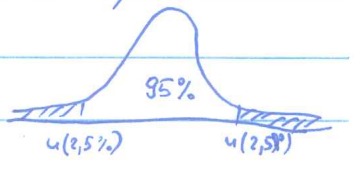
\includegraphics[width=0.3\textwidth]{imgs/obr25.png}
	\end{multicols}
	\end{itemize}
\end{enumerate}

\begin{align*}
95\% &= P(-u(2.5\%) < \frac{Z-atanh/\rho)}{\sqrt{\frac{1}{n-3}}} < u(2.5\%))\\
&= P(Z-u(2.5\%)\sqrt{\frac{1}{n-3}} < atanh(\rho) < Z+u(2.5\%)\frac{1}{n-3})\\
&= P(tanh(Z-u(2.5\%)\sqrt{\frac{1}{n-3}}) < \rho < tanh(Z+u(2.5\%)\frac{1}{n-3}))
\end{align*}

$\qquad \to$ tanh je rastúca funckia $\to$ môžeme použiť

\underline{$IS = (0.41, 0.76)$} nie je symetrický

POZN: je niečo ako Z-prem pre SPEARMANA $\sim N(\ldots, \frac{1.06}{n-3})$, nie pre ľubovoľné rozdelenie

\subsubsection*{2-sample test}
$\left(\begin{matrix}
  X\\
  Y
 \end{matrix}\right)\begin{matrix}
  - & INCOME\\
  - & HS.grad
 \end{matrix}$
 
\begin{align*}
JUH: \hat{\rho}_1 &= 0.83 \qquad &SEVER:~ &\hat{\rho}_2 = 0.20 \\
\rho_1 &= ~? &\qquad &\rho_2 = ~?
\end{align*}
$$H_0: \rho_1 = \rho_2 \qquad vs. \qquad H_1: \rho_1 \neq \rho_2$$
$$Z_1 \dot{\sim} N(atanh(\rho_1), \frac{1}{n_1-3}) \qquad Z_2 \dot{\sim} N(atanh(\rho_2, \frac{1}{n_2-3})$$

$Z_1, Z_2$ \underline{sú nezavíslé} $\Rightarrow$\footnote{z nezávislosti aj z predošlého riadku} $Z_1-Z_2 ~\dot{\sim}~ N(atanh(\rho_1)-atanh(\rho_2), \frac{1}{n_1-3} + \frac{1}{n_2+3})$

\begin{align*}
\Aboxed{\frac{(Z_1-Z_2) - (atanh(\rho_1) - atanh(\rho_2))}{\sqrt{\frac{1}{n_1-3} + \frac{1}{n_2-3}}} ~\dot{\sim}~ N(0,1)}
\end{align*}

$\qquad \Rightarrow$ TESTOVÁ ŠTATISTIKA $\frac{Z_1 - Z_2}{\sqrt{\frac{1}{n_1-3}+\frac{1}{n_2-3}}} =: Z_{1,2}$, porovnáme s $u(2.5\%)$.

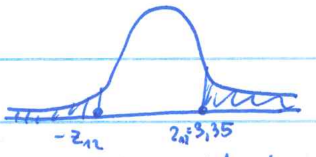
\includegraphics[width=0.3\textwidth]{imgs/obr26.png}

$p-val\qquad2(1-prnom(Z_{1,2})) < 5\% \Rightarrow H_0$ zamietame

\textbf{TEÓRIA:} SEVER: aj nevzdelaní si vedia zarobiť -- lepší systém, JUH: nevzdelaní sú kopáči

\section*{Lineárna regresia}
$Y_i = \beta_0 + \beta_1x_i + \varepsilon_i \qquad \varepsilon_i \sim N(0, \sigma^2), i = 1\ldots n$

$Y_i$ -- ozón,$\beta_0 = ~?, \beta_1 = ~?$ -- parametre regresie, $x_i$ -- teplota, $\varepsilon_i$ -- chyba regres. modelu

\begin{align*}
\left(\begin{matrix}
  Y_1\\
  \vdots\\
  Y_n
 \end{matrix}\right)
 &=
\left(\begin{matrix}
  1 & X_1\\
  \vdots & \vdots\\
  1 & X_n
 \end{matrix}\right) 
\left(\begin{matrix}
  \beta_0\\
  \beta_1
 \end{matrix}\right)  
 +
\left(\begin{matrix}
  \varepsilon_1\\
  \vdots\\
  \varepsilon_n
 \end{matrix}\right)\\
\vec{Y} &= \mathbf{X}\vec{\beta} + \vec{\varepsilon} 
\end{align*}

Chceme zistiť $\beta = \binom{\beta_0 = ~?}{\beta_1 = ~?} \to$ treba ich odhadnúť.

LS-estimator -- LEAST SQUARES $\to$ súčet zvislých odchýlok = 0, súčet štvorcov.

odchýlky = reziduá \qquad $\hat{\beta} = (X^TX)^{-1}X^TY$

$$
\begin{matrix}
  \hat{\beta_0} =\\
  \hat{\beta_1} =
 \end{matrix} 
\left(\begin{matrix}
  -2.22\\
  0.07
 \end{matrix}\right)
 = \hat{\beta}
$$

KONTRAST: $a_0\beta_0 + a_1\beta_1 = (a_0, a_1)\binom{\beta_0}{\beta_1} = a^T\beta = ?$

ODHAD PRE KONTRAST: $a^T\hat{\beta}$ \qquad PLATÍ $\frac{a^T\hat{\beta} - a^T\beta}{S\sqrt{a^T(X^TX)^{-1}a}} \sim t_{n-2}$

$t_{n-2}$ -- n-\textbf{2} lebo v modeli sú 2 parametre $\beta$

$S$ -- odhad pre $\sigma \to$ smerodajná odchýlka chýb. $S^2 = \frac{SS_e}{n-2}, \qquad SS_e = \sum_{i=1}^n(reziduum)^2 = \sum_{i=1}^n \varepsilon_i^2$, SUM of SQUARES (zase n-2, lebo 2 bety)

$\qquad \to$ z toho dostaneme MMS IS pre $\beta$

\vspace{20mm}

\begin{multicols}{2}

\textbf{IS pre $a^T\beta$}:  \encircle{1} $a^T\hat{\beta} \pm t_{n-2}(2.5\%)\cdot S\sqrt{a^T(X^TX)^{-1}a}$

$$reziduum = \left(\begin{matrix}
Y_1 - (\hat{\beta_0} + \hat{\beta}_1x_1) \\
\vdots\\
Y_n - (\hat{\beta_0} + \hat{\beta}_1x_n)
\end{matrix}\right)
= \vec{Y}-\vec{X}\hat{\beta}$$

$\beta_1 = ~?$ -- nepoznáme
\begin{enumerate}
\item bodový odhad $\hat{\beta}_1 = 0.07$ (lin. regres)
\item $(0,1)\binom{\beta_0}{\beta_1} = \beta_1$ -- do IS pre kontrast vložíme vektor (0,1)
\end{enumerate}

$x = 85^\circ F (29.4^\circ C) \Rightarrow E(Y)=~Y$

$E(Y) = E(\beta_0 + \beta_1\cdot85 + \varepsilon) = \beta_0 + \beta_1\cdot85 + E(\varepsilon) = ~?$

\columnbreak

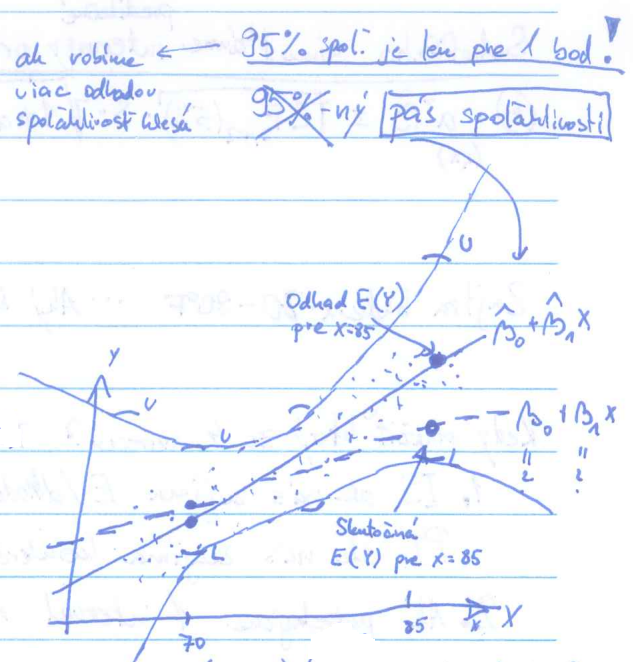
\includegraphics[width=0.4\textwidth]{imgs/obr27.png}

\end{multicols}

\begin{enumerate}
\item Bodový odhad dosadíme za $\beta_0, \beta_1$ odhady $\hat{\beta}_0, \hat{\beta}_1 \Rightarrow \hat{\beta}_0 + \hat{\beta}_1\cdot85 = (1,85)\binom{\hat{\beta}_0}{\hat{\beta}_1} = 3.75$, kontrast = (1,85)
\item Intervalový odhad pre $E(Y): (3.61, 3.89) = (L,U)$

$E$ - str. hodnota -- zo zákona veľkých čísel -- ak veľakrát zopakujeme pokus, $\bar{Y} \to E(Y)$
\end{enumerate}

\textbf{Scheffeho simultanne inetrvaly spoľahlivosti pre $a^T\beta$}
\vspace{5mm}

\encircle{2} $a^T\hat{\beta} \pm \sqrt{2F_{2,n-2}(5\%)}S\sqrt{a^T(X^TX)^{-1}a}$ -- 95\% určujú pás spoľahlivosti

Všetky dvojky v $2F_{2,n-2}$ sú \# parametrov. $F$ je Fischer-Schnedeker. 

rozširovanie na okrahoch: v strede je veľa dát(istejší), na krajoch je menej (menej istý odhad)

\subsection*{Predikčný interval}
Zajtra bude $85^\circ F$ \ldots aký bude ozón?	\qquad $Y = ~? = \beta_0 + \beta_1\cdot85 + \varepsilon$
\begin{enumerate}
\item Bodový odhad $\hat{\beta}_0 + \hat{\beta}_1\cdot85 + 0$
\item Intervalový odhad = PREDIKČNÝ INTERVAL \encircle{3} $a^T\hat{\beta} \pm t_{n-2}(2.5\%)\sqrt{1+a^T(X^TX)^{-1}a}$
\end{enumerate}

\textbf{POZN1:} PI pre $Y$\footnote{$Y = \beta_0+\beta_1\cdot85 + \varepsilon \leftarrow$ 3 zdroje neistoty }: (2.58, 4.92) \qquad IS pre $E(Y)$\footnote{$E(Y) = \beta_0 + \beta_1\cdot85 \leftarrow$ 2 zdroje neistoty}: (3.61, 3.89)

$\qquad \to$ Prečo je Pi širší? -- suchý dôvod: lebo je vo vzorci $1+$, -- berie do úvahu $\varepsilon$

\textbf{POZN2}: Čo je predikčný interval?

\begin{multicols}{2}

``chytanie medveďa'':\\
P(teplota zajtra padne do PI) = 95\%

``chytanie motýľa'':\\
P(odhad IS trafí skutočnú hodnotu $E(Y)$)

\columnbreak

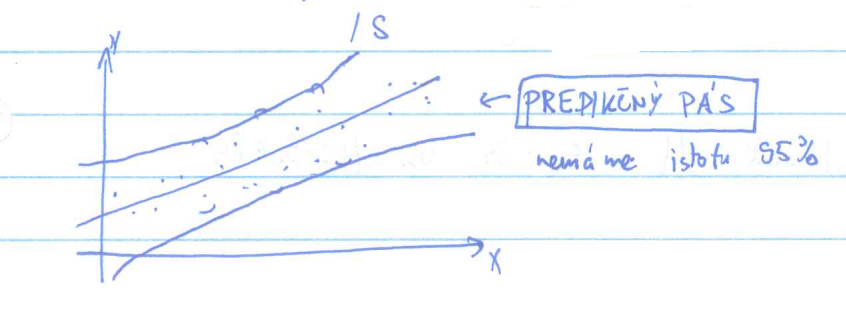
\includegraphics[width=0.4\textwidth]{imgs/obr28.png}
\end{multicols}


\begin{multicols}{2}

~\\
\textbf{Scheffeho simultánne predikčné intervaly pre Y}

\encircle{4} $a^T\hat{\beta} \pm \sqrt{2F_{2,n-2}(5\%)S\sqrt{1+a^T(X^TX)^{-1}a}}$

Zajtra bude $x = 70 - 80^\circ F$ \ldots Aký bude ozón?

\columnbreak

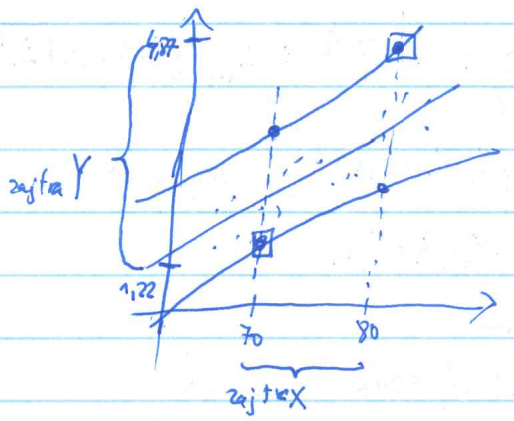
\includegraphics[width=0.3\textwidth]{imgs/obr29.png}

\end{multicols}

Kedy použiť ktorý zo 4 vzorcov? treba to mať natrénované.
\begin{enumerate}
\item IS ak nás zaujíma $E$/dlhodobý priemer/parameter\\
PI ak nás zaujíma konkrétna hodnota
\item Ak potrebujeme 1 inetrval $\to$ 1/3, AK potrebujeme viac intervalov naraz $\to$ Scheffe
\end{enumerate}

\subsection*{Polynomická regresia}
$Y_i = \beta_0 + \beta_1x_i + \beta_2x_i^2 + \varepsilon_i \qquad \varepsilon_i \sim N(0, \sigma^2)$

Kde: $\sigma^2 = ~?$, $Y = $ ventilation -- ako pumpujú pľúca, $x_i$ -- oxygen -- koľko kyslíka z neho vedia vytiahnuť.

$$\hat{\beta}_0 = 24.27 \qquad \hat{\beta_1} = -0.01344 \qquad \hat{\beta}_2 = 0.000008902$$

Vo vzorcoch 1-4 teraz použijeme \# parametrov 3. $a = (1, x, x^2)^T$

\textbf{TEST OF SIGNIFICANCE OF $\beta_2$}: \underline{Chceme zjednodušiť model} $\to$ zanedbať parameter $\hat{\beta}_2$

$$H_0: \beta_2 = 0 \qquad vs. \qquad H_1: \beta_2 \neq 0$$

$$\beta_2 = (0,0,1)\left(\begin{matrix}
\beta_0\\
\beta_1\\
\beta_2
\end{matrix}\right), \qquad a^T = (0,0,1)$$

$$\frac{a^T\hat{\beta} - a^T\beta}{S\sqrt{a^T(X^TX)^{-1}a}} \sim t_{n-3}$$
$$T = \frac{a^T\hat{\beta} - 0}{S\sqrt{a^T(X^TX)^{-1}a}}$$

$H_0$ zamietame ak $\hat{\beta}_2 >> 0$ alebo ak $\hat{\beta}_2 << 0$.

\begin{enumerate}
\item $\hat{\beta}_2$ je malé, lebo $x-y$ sú veľké (1000) $\to$ $x^2$ je $10^6 \to$ ale $\beta_2$ je dôležité
\item $\beta_2$ je potrebné, lebo obrázok 
\end{enumerate}

\subsubsection*{Summary}
\begin{itemize}
\item call -- akým príkazom vznikol objekt
\item residuals -- zvislé odchýlky
\item coefficients:
	\begin{itemize}
	\item stderror -- menovateľ T
	\item t value -- test. štatistika T
	\item p-value pre T: $2\cdot 10^{-16} < 5\% \Rightarrow H_0$ brutálne zamietame
	\end{itemize}
\item residual standard error = S, \texttt{\$sigma}
\item Test. štatistiku, že $H_0: \beta_0 = 24 ~vs.~ H_1: \beta_0 \neq 24$ už nedostaneme zo summary $\Rightarrow$ ručne
\end{itemize}

Porcelán -- výsk. ústav zváračský cestou do Rače\\
-- odolnosť porc. voči vysokým teplotám -- teplotné šoky \qquad teplota1 -- 1. šok, potom schladenie, potom 2. šok, potom zmerali pnutie doštičky\\
--ako teplotné šoky vplývajú na pnutie

$Y = \beta_0 + \beta_1x_1 + \beta_2x_2 + \varepsilon$, $Y$ -- napätie, $x_1$ -- teplota 1. šoku, $x_2$ -- teplota 2.šoku

$\hat{\beta}_0 = 2.62 \qquad \hat{\beta}_1 = 0.05776 \qquad \hat{\beta}_2 = 0.05667$ je model dobrý?

\begin{multicols}{2}

~\\
12 dát, 12 guličiek + prekladáme cez ne rovinu\\
3D obrázok by sme vedeli nakresliť, 4D si už nechceme ani predstavovať\\
$\qquad \to$ \underline{chceme zistiť, či je model dobrý ``pomocou číselka''}

\columnbreak

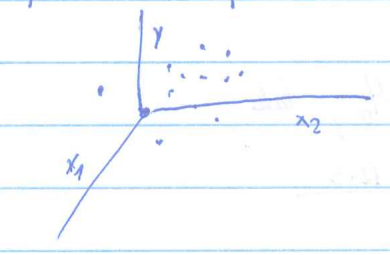
\includegraphics[width=0.3\textwidth]{imgs/obr30.png}

\end{multicols}

\begin{multicols}{2}

``krásu'' odmeriame pomocou $SS_e$\\
$SS_e = $ \textbf{miera nekvality modelu}

\columnbreak

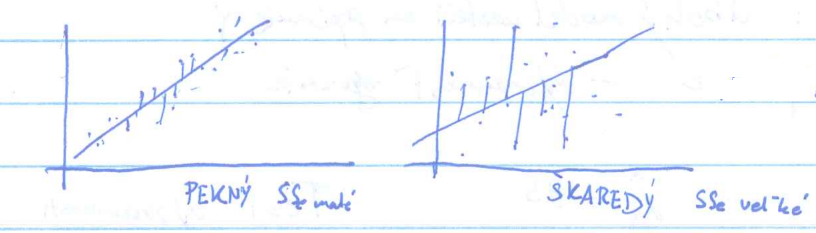
\includegraphics[width=0.4\textwidth]{imgs/obr31.png}

\end{multicols}

Aby sme $SS_e$ vedeli porovnať, vytvoríme ÚBOHÝ MODEL(null model) $Y = \beta_0 + \varepsilon$ + ztrátame (total) $SS_t$

ÚBOHÝ MODEL JE URČITE NEKVALITNEJŠÍ $\Rightarrow$ $SS_t \geq SS_r$
\begin{itemize}
\item[a)] $X_1, X_2$ sú dôležité na určenie $y$ $\Rightarrow$ úbohý model bude oveľa horší než náš $SS_t >> SS_e \qquad \frac{SS_e}{SS_t} \dot{=} 0$
\begin{align*}
R^2 = \Aboxed{1-\frac{SS_e}{SS_t}} \dot{=}1
\end{align*}
\item[b)] $X_1, X_2$ nie sú dôležité na určenie $y$ $\Rightarrow$ úbohý model nebude oveľa horší než náš $SS_t \dot{=} SS_e \qquad \frac{SS_e}{SS_t} \dot{=} 1$
\begin{align*}
R^2 = \Aboxed{1-\frac{SS_e}{SS_t}} \dot{=}0
\end{align*}
\end{itemize}

učenie -- determinovanie -- $R^2$ = \textbf{KOEFICIENT DETERMINÁCIE} (ako veľmi sú $x$-y potrebné na určenie $Y$

\underline{summary}: multiple R-squared \$r.squared
\vspace{5mm}

Ale: mnohé znaky nekvality sa pomocou $R^2$ zistiť nedajú (ale $R^2$ je najslávnejší, lebo Excel vedel spočítať $\hat{\beta}$ a $R^2$)
\vspace{5mm}

Ktorý šok má vyšší vplyv na napätie \ldots ak veríme modelu, je to určené $\beta_1$ a $\beta_2$
$$H_0: \beta_1 \leq \beta_2 \qquad vs. \qquad H_1: \beta_1 > \beta_2$$
MZR: $H_0$ zamietame ak $\hat{\beta}_1 >> \hat{\beta}_2$, $\hat{\beta}_1 - \hat{\beta}_2 >> 0$, $(0,1,-1)\hat{\beta} >> 0$. Použijeme test pre kontrasty:
$$T = \frac{a^T\hat{\beta}-0}{S\sqrt{a^T(X^TX)^{-1}a}}$$
$H_0$ zamietame ak $T >> 0$.\\
$H_0$ sme nezamietli $\to$ test pvoedal, že nevieme povedať že $\beta_1$ je dôležitejšia $\Rightarrow$ málo dát, pomerne malý rozdiel

\subsection*{Test významnosti regresie}
$$Y = \beta_0 + \beta_1x_1 + \beta_2x_2 + \varepsilon \to SS_e$$
$$H_0: \beta_1 = 0 \land \beta_2 = 0 \qquad vs. \qquad H_1: \beta_1 \neq 0 \lor \beta_2 \neq 0$$

$H_1$ hovorí, že úbohý nestačí, $H_0$ hovorí, že úbohý model stačí na popísanie $Y$

Úbohý mdoel $Y = \beta_0 + \varepsilon \to SS_t$.

$H_0$ zamietame ak: $SS_t >> SS_e$, teda ak:
$$F = \frac{\frac{SS_t-SS_e}{2}}{\frac{SS_e}{n-3}} >> 0 \qquad F \sim F_{2,n-3}$$

Kde, 2 znamená počet zabitých biet, a š znamená počet biet v pôvodnom modeli. Menovateľ veľkého zlomku je $S^2 = \frac{SS_e}{n-3}$.

$p-value \dot{=} 5\% \Rightarrow H_0$ zamietame: úbohý mdoel nestačí na popísanie $Y$

\underline{summary}: F-statistic = test. štatistika + p-value -- významnosť regresie
\vspace{5mm}

$Y = \alpha_0 + \alpha_1t_1 + \alpha_2t_2 + \varepsilon$, kde $Y$ je napätie, $t_1$ je trvanie 1. šoku, $t_2$ je trvanie 2. šoku
$$\hat{\alpha}_0 = 93 \qquad \hat{\alpha}_1 = 0.01992 \qquad \hat{\alpha}_2 = 0.02227$$
Test významnosti: $H_0: \alpha_1 = 0 \land \alpha_2 = 0 ~vs.~ H_1: \alpha_1 \neq 0 \lor \alpha_2 \neq 0$. $T = 0.92$, $p-value = 41\% \Rightarrow H_0$ nezamietame. $R^2 = 0.17 << 1$

\subsection*{Testovanie hypotézy o submodeli}
$Y = \beta_0 + \beta_1x_1 + \beta_2x_2 + \beta_3x_3 \Rightarrow SS_{e,model}$, kde $Y$ je ozone, $x_1$ je radiation, $x_2$ je temp, $x_3$ je wind.
$$\hat{\beta}_0 = -0.297\qquad \hat{\beta}_1 = 0.002206\qquad \hat{\beta}_2 = 0.05\qquad \hat{\beta}_3 = -0.076$$
$$H_0: \beta_0 = 0 \land \beta_1 = 0 \qquad vs. \qquad H_1: \beta_0 \neq 0 \lor \beta_1 \neq 0$$
$H_0$ -- submodel stačí, $H_1$ -- submodel nestačína popísanie $Y$\\
Submodel: zohľadňuje $H_0: Y = \beta_2x_2 + \beta_3x_3 + \varepsilon \Rightarrow SS_{e,submodel}$

\begin{multicols}{2}

MZR: $H_0$ zamietame ak $SS_{e,submodel} >> SS_{e,model}$ \ldots $SS_{e,submodel} - SS_{e,model} >> 0$:
$$F= \frac{\frac{SS_{e,submodel}-SS_{e,model}}{2}}{\frac{SS_{e,model}}{n-4}} \sim F_{2,n-4}$$

$F = 8.06$, $p-value = 1-pF(2,n-4) = 0.05 < 5\% \Rightarrow H_0$ zamietame -- nemôžeme naraz vyhodiť $\beta_0$ aj $\beta_1$

\columnbreak

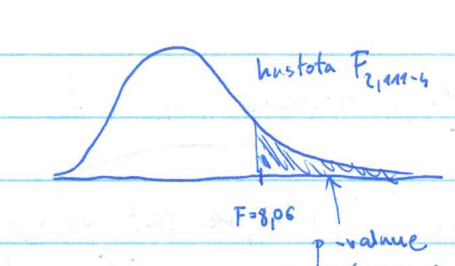
\includegraphics[width=0.4\textwidth]{imgs/obr32.png}

\end{multicols}

*alternatívny postup:
\begin{enumerate}
\item $H'_0: \beta_0 = 0 ~vs.~ H'_1: \beta_0 \neq 0$ (test hypotézy o kontraste) $\to$ 5\% error typu I.
\item $H''_0: \beta_1 = 0 ~vs.~ H''_1: \beta_1 \neq 0$ (test hypotézy o kontraste) $\to$ 5\% error typu I.
\end{enumerate}
pravidlo: $H_0$ zamietame ak zamietame $H'_0$ alebo $H''_0$ $\to$ chyba I. druhu s $p > 5\%$.

!!! Nedeliť test na viacero, ak sa dá otestovať všetko jedným testom na hladine $5\%$, použiť ten.

\subsection*{Regresná diagnostika (stručný úvod)}
-- ako sprojektovať veľarozmerný priestor do $\mathcal{R}^2$, aby sme vedeli zistiť, ako dobre regresia funguje.

\subsubsection*{which=1: Residuals vs. Fitted values}
-- os x: fitted values = odhadované hodnoty $\hat{\beta}_0 + \hat{\beta}_1x_{1i} + \hat{\beta}_2x_{2i} + \hat{\beta}_3x_{3i}$ (111 čísel)

-- os y: residuals = $Y$ fitované hodnoty (111 čísel)

ideál: 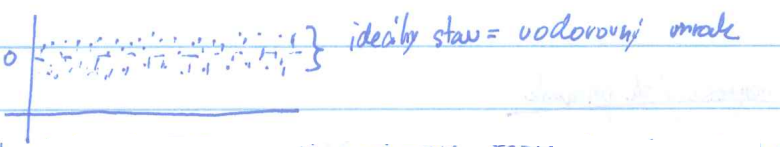
\includegraphics[width=0.3\textwidth]{imgs/obr33.png}

\begin{multicols}{2}

\begin{itemize}
\item označené dni \underline{20,23,77} majú najvyššie reziduá $\to$ sú podozrivé
\item ak sú oblasti celé nad/pod $\to$ systematické chyby
\item rozšírené niektoré oblasti

	-- veľký rozpor s $\varepsilon_i \sim N(0, \sigma^2)$
	
	-- $\forall \varepsilon$ by mali byť z rovnakého rozdelenia
	
	$D(\varepsilon_i)$ je konštantná -- HOMOSCEDASTICITY
	
	HETEROSCEDASTICITY-- teória je celá založená na konšt. $\to$ veľký problém
\end{itemize}

\columnbreak

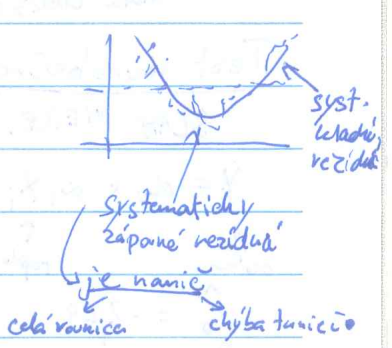
\includegraphics[width=0.3\textwidth]{imgs/obr34.png}

\vspace{5mm}

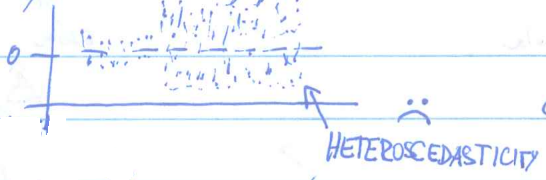
\includegraphics[width=0.3\textwidth]{imgs/obr35.png}

\end{multicols}

\subsubsection*{which=3: Scale-location}
-- absolútne hodnoty reziduí, odmocníme, znormalizujeme, tiež by mal vyzerať ako vodorovný mrak

\subsubsection*{which=2: Normal Q-Q}

\begin{multicols}{2}

$\varepsilon_1, \ldots, \varepsilon_n \overset{?}{\sim} N(,)$

-- my ich nepoznáme, nie sú to \textbf{rezisuá} (ale náh. premenné -- odchýlky od skut. regresnej priamky)

--odhadneme $\varepsilon$ pomocou $\hat{\varepsilon}_1, \ldots, \hat{\varepsilon}_n$ (residuals)

--otestujeme $\hat{\varepsilon}_1, \ldots, \hat{\varepsilon}_n \overset{?}{\sim} N()$ -- obrázok / \texttt{ks.test}

\columnbreak

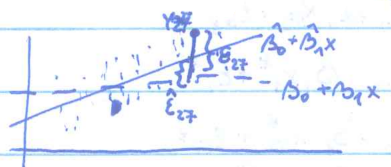
\includegraphics[width=0.5\textwidth]{imgs/obr36.png}

\end{multicols}

\underline{Čo ak zamietame normalitu?} ak $\varepsilon$ nemajú norm. rozdelenie
\begin{enumerate}
\item $\hat{\beta} = LS-ESTIMATOR$ od $\beta$ \checkmark -- funguje bez ohľadu na normálne rozdenenie $\varepsilon$, len iid
\item IS, pásy, PI, predikčné pásy, testy -- \texttimes -- toto nefunguje, treba použiť náhradné metódy -- nezaručujú 95\%
\end{enumerate}

\subsubsection*{which=4: Cook's distance}
-- ako veľmi konkrétne body ovplyvňujú regresiu
\begin{itemize}
\item[a)]
\begin{multicols}{2}

COOK'S DISTANCE$_{14} = \sum_{i=1}^n(\updownarrow)^2$\\
ak bol $Y_{14}$ outlier $\to$ je to vysoké číslo

\columnbreak

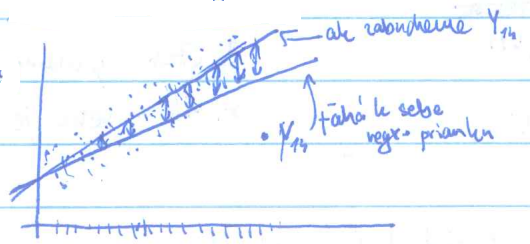
\includegraphics[width=0.4\textwidth]{imgs/obr37.png}

\end{multicols}

\item[b)]
\begin{multicols}{2}

COOK'S DISTANCE$_{25} = \sum_{i=1}^n(\updownarrow)^2$\\
ak nebol $Y_{25}$ outlier $\to$ je to malé číslo

\columnbreak

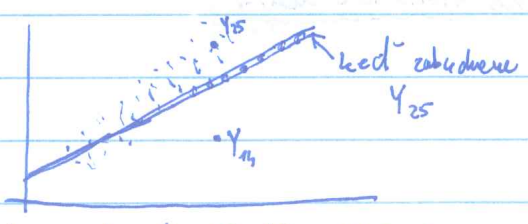
\includegraphics[width=0.4\textwidth]{imgs/obr38.png}

\end{multicols}

\end{itemize}

Pre body, ktoré majú vysokú COOK'S DISTANCE treba skúsiť dáta vyhodiť, ak sa veľmi zmenia $\hat{\beta}$ (zmenia znamienka) $\to$ zmena interpretácie

Podľa Cooka sú podozrivé dáta \underline{17,30,77}.

\vspace{5mm}
Veľké rezíduum $\nRightarrow$ Veľké Cook's distance

Veľké Cook's distance $\nRightarrow$ Veľké rezíduum

\begin{multicols}{2}

\textbf{LEVERAGE POINT} ( vplyvný bod )\\
$\qquad \to$ treba hľadať pomocou Cook's dostance

\columnbreak

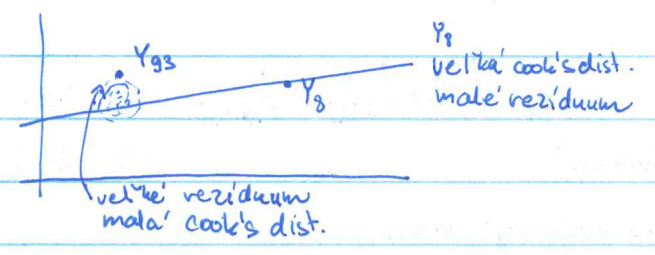
\includegraphics[width=0.4\textwidth]{imgs/obr39.png}

\end{multicols}


\subsection*{Test rovnobežnosti regresných priamok}

\begin{multicols}{2}

\begin{center}
SLABÝ VIETOR
$$Y_i = \alpha_0 + \alpha_1x_i + \varepsilon_i \qquad (i=1,\ldots,58)$$
$Y_i$ -- ozón, $x_i$ -- teplota
$$\hat{\alpha}_0 = -2.69$$
$$\hat{\alpha}_1 = 0.078$$
\end{center}

\columnbreak

\begin{center}
SILNÝ VIETOR
$$Y^*_i = \beta_0 + \beta_1x^*_i + \varepsilon^*_i \qquad (i=1,\ldots,53)$$
$Y^*_i$ -- ozón, $x^*_i$ -- teplota
$$\hat{\beta}_0 = -0.35$$
$$\hat{\beta}_1 = 0.04$$
\end{center}

\end{multicols}

Zdá sa nám, že silný vietor znižuje ozón za rovnakej teploty
$$H_0: \alpha_1 \leq \beta_1 \qquad vs. \qquad H_1: \alpha_1 > \beta_1$$

\subsubsection*{Zložený model}

\begin{align*}
\left(\begin{matrix}
Y_1\\
\vdots\\
Y_{58}\\
--\\
Y^*_1\\
\vdots\\
Y^*_{53}
\end{matrix}\right)
&=
\left(\begin{matrix}
1 & 0 & x_1 & 0\\
\vdots & \vdots & \vdots & \vdots \\
1 & 0 & x_{58} & 0\\
--&--&--&--\\
0 & 1 & 0 & x^*_1\\
\vdots & \vdots & \vdots & \vdots \\
0 & 1 & 0 & x^*_{53}
\end{matrix}\right)
\cdot
\left(\begin{matrix}
\alpha_0\\
\beta_0\\
\alpha_1\\
\beta_1
\end{matrix}\right)
+
\left(\begin{matrix}
\varepsilon_1\\
\vdots\\
\varepsilon_{58}\\
--\\
\varepsilon^*_1\\
\vdots\\
\varepsilon^*_{53}
\end{matrix}\right) \\ 
Y &= X\cdot\gamma + 
\end{align*}

\begin{align*}
Y_1 &= \alpha_0 + \alpha_1x_1 + \varepsilon_1\\
\vdots\\
Y_{58} &= \alpha_0 + \alpha_1x_{58} + \varepsilon_{58}\\
Y^*_1 &= \beta_0 + \beta_1x^*_1 + \varepsilon^*_1\\
\vdots\\
Y^*_{53} &= \beta_0 + \beta_1x^*_{53} + \varepsilon^*_{53}
\end{align*}

Vyjde $\hat{\gamma}^T = (\hat{\alpha}_0, \hat{\beta}_0, \hat{\alpha}_1, \hat{\beta}_1)$.

\vspace{5mm}
Máme 1 model, môžeme robiť test:
$$H_0: \alpha_1 \leq \beta_1 \Leftrightarrow \alpha_1 - \beta_1 \leq 0 \qquad \Rightarrow \mathrm{test~o~kontraste~}a = (0,0,1,-1)$$

\begin{multicols}{2}

$$T = \frac{a^T\hat{\gamma} - a^T\gamma}{S\sqrt{a^T(X^TX)^{-1}a}}$$
kde, $a^T\hat{\gamma} = \hat{\alpha}_1 - \hat{\beta}_1$ a $a^T\gamma = 0$.\\
$H_0$ zamietame ak $\alpha_1 - \beta_1 >> 0 \Rightarrow T >> 0$.\\
$p-val = 0.1\% < 5\% \Rightarrow H_0$ zamietame.

\columnbreak

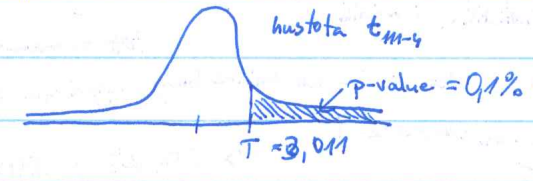
\includegraphics[width=0.4\textwidth]{imgs/obr40.png}

\end{multicols}

Je štatisticky významné, že pri silnom vetre je nižší ozón.

\end{document}